\documentclass[
  shownotes,
  xcolor={svgnames},
  hyperref={colorlinks,citecolor=DarkBlue,linkcolor=DarkRed,urlcolor=DarkBlue}
  , aspectratio=169]{beamer}
\usepackage{animate}
\usepackage{amsmath}
\usepackage{amsfonts}
\usepackage{amssymb}
\usepackage{pifont}
\usepackage{mathpazo}
%\usepackage{xcolor}
\usepackage{multimedia}
\usepackage{fancybox}
\usepackage[para]{threeparttable}
\usepackage{multirow}
\setcounter{MaxMatrixCols}{30}
\usepackage{subcaption}
\usepackage{graphicx}
\usepackage{lscape}
\usepackage[compatibility=false,font=small]{caption}
\usepackage{booktabs}
\usepackage{ragged2e}
\usepackage{chronosys}
\usepackage{appendixnumberbeamer}
\usepackage{animate}
\setbeamertemplate{caption}[numbered]
\usepackage{color}
%\usepackage{times}
\usepackage{tikz}
\usepackage{comment} %to comment
%% BibTeX settings
\usepackage{natbib}
\bibliographystyle{apalike}
\bibpunct{(}{)}{,}{a}{,}{,}
\setbeamertemplate{bibliography item}{[\theenumiv]}

% Defines columns for bespoke tables
\usepackage{array}
\newcolumntype{L}[1]{>{\raggedright\let\newline\\\arraybackslash\hspace{0pt}}m{#1}}
\newcolumntype{C}[1]{>{\centering\let\newline\\\arraybackslash\hspace{0pt}}m{#1}}
\newcolumntype{R}[1]{>{\raggedleft\let\newline\\\arraybackslash\hspace{0pt}}m{#1}}


\usepackage{xfrac}


\usepackage{multicol}
\setlength{\columnsep}{0.5cm}

% Theme and colors
\usetheme{Boadilla}

% I use steel blue and a custom color palette. This defines it.
\definecolor{andesred}{HTML}{af2433}

% Other options
\providecommand{\U}[1]{\protect\rule{.1in}{.1in}}
\usefonttheme{serif}
\setbeamertemplate{itemize items}[default]
\setbeamertemplate{enumerate items}[square]
\setbeamertemplate{section in toc}[circle]

\makeatletter

\definecolor{mybackground}{HTML}{82CAFA}
\definecolor{myforeground}{HTML}{0000A0}

\setbeamercolor{normal text}{fg=black,bg=white}
\setbeamercolor{alerted text}{fg=red}
\setbeamercolor{example text}{fg=black}

\setbeamercolor{background canvas}{fg=myforeground, bg=white}
\setbeamercolor{background}{fg=myforeground, bg=mybackground}

\setbeamercolor{palette primary}{fg=black, bg=gray!30!white}
\setbeamercolor{palette secondary}{fg=black, bg=gray!20!white}
\setbeamercolor{palette tertiary}{fg=white, bg=andesred}

\setbeamercolor{frametitle}{fg=andesred}
\setbeamercolor{title}{fg=andesred}
\setbeamercolor{block title}{fg=andesred}
\setbeamercolor{itemize item}{fg=andesred}
\setbeamercolor{itemize subitem}{fg=andesred}
\setbeamercolor{itemize subsubitem}{fg=andesred}
\setbeamercolor{enumerate item}{fg=andesred}
\setbeamercolor{item projected}{bg=gray!30!white,fg=andesred}
\setbeamercolor{enumerate subitem}{fg=andesred}
\setbeamercolor{section number projected}{bg=gray!30!white,fg=andesred}
\setbeamercolor{section in toc}{fg=andesred}
\setbeamercolor{caption name}{fg=andesred}
\setbeamercolor{button}{bg=gray!30!white,fg=andesred}


\usepackage{fancyvrb}
\newcommand{\VerbBar}{|}
\newcommand{\VERB}{\Verb[commandchars=\\\{\}]}
\DefineVerbatimEnvironment{Highlighting}{Verbatim}{commandchars=\\\{\}}
% Add ',fontsize=\small' for more characters per line
\usepackage{framed}
\definecolor{shadecolor}{RGB}{248,248,248}
\newenvironment{Shaded}{\begin{snugshade}}{\end{snugshade}}
\newcommand{\AlertTok}[1]{\textcolor[rgb]{0.94,0.16,0.16}{#1}}
\newcommand{\AnnotationTok}[1]{\textcolor[rgb]{0.56,0.35,0.01}{\textbf{\textit{#1}}}}
\newcommand{\AttributeTok}[1]{\textcolor[rgb]{0.77,0.63,0.00}{#1}}
\newcommand{\BaseNTok}[1]{\textcolor[rgb]{0.00,0.00,0.81}{#1}}
\newcommand{\BuiltInTok}[1]{#1}
\newcommand{\CharTok}[1]{\textcolor[rgb]{0.31,0.60,0.02}{#1}}
\newcommand{\CommentTok}[1]{\textcolor[rgb]{0.56,0.35,0.01}{\textit{#1}}}
\newcommand{\CommentVarTok}[1]{\textcolor[rgb]{0.56,0.35,0.01}{\textbf{\textit{#1}}}}
\newcommand{\ConstantTok}[1]{\textcolor[rgb]{0.00,0.00,0.00}{#1}}
\newcommand{\ControlFlowTok}[1]{\textcolor[rgb]{0.13,0.29,0.53}{\textbf{#1}}}
\newcommand{\DataTypeTok}[1]{\textcolor[rgb]{0.13,0.29,0.53}{#1}}
\newcommand{\DecValTok}[1]{\textcolor[rgb]{0.00,0.00,0.81}{#1}}
\newcommand{\DocumentationTok}[1]{\textcolor[rgb]{0.56,0.35,0.01}{\textbf{\textit{#1}}}}
\newcommand{\ErrorTok}[1]{\textcolor[rgb]{0.64,0.00,0.00}{\textbf{#1}}}
\newcommand{\ExtensionTok}[1]{#1}
\newcommand{\FloatTok}[1]{\textcolor[rgb]{0.00,0.00,0.81}{#1}}
\newcommand{\FunctionTok}[1]{\textcolor[rgb]{0.00,0.00,0.00}{#1}}
\newcommand{\ImportTok}[1]{#1}
\newcommand{\InformationTok}[1]{\textcolor[rgb]{0.56,0.35,0.01}{\textbf{\textit{#1}}}}
\newcommand{\KeywordTok}[1]{\textcolor[rgb]{0.13,0.29,0.53}{\textbf{#1}}}
\newcommand{\NormalTok}[1]{#1}
\newcommand{\OperatorTok}[1]{\textcolor[rgb]{0.81,0.36,0.00}{\textbf{#1}}}
\newcommand{\OtherTok}[1]{\textcolor[rgb]{0.56,0.35,0.01}{#1}}
\newcommand{\PreprocessorTok}[1]{\textcolor[rgb]{0.56,0.35,0.01}{\textit{#1}}}
\newcommand{\RegionMarkerTok}[1]{#1}
\newcommand{\SpecialCharTok}[1]{\textcolor[rgb]{0.00,0.00,0.00}{#1}}
\newcommand{\SpecialStringTok}[1]{\textcolor[rgb]{0.31,0.60,0.02}{#1}}
\newcommand{\StringTok}[1]{\textcolor[rgb]{0.31,0.60,0.02}{#1}}
\newcommand{\VariableTok}[1]{\textcolor[rgb]{0.00,0.00,0.00}{#1}}
\newcommand{\VerbatimStringTok}[1]{\textcolor[rgb]{0.31,0.60,0.02}{#1}}
\newcommand{\WarningTok}[1]{\textcolor[rgb]{0.56,0.35,0.01}{\textbf{\textit{#1}}}}
\usepackage{graphicx}
\makeatletter


% colors
\definecolor{airforceblue}{rgb}{0.36, 0.54, 0.66}
\newcommand{\theme}{\color{andesred}}
\newcommand{\bk}{\color{black}}
\newcommand{\rd}{\color{red}}
\newcommand{\fg}{\color{ForestGreen}}
\newcommand{\bl}{\color{blue}}
\newcommand{\gr}{\color{black!60}}
\newcommand{\sg}{\color{DarkSlateGray}}
\newcommand{\br}{\color{SaddleBrown}}
\newcommand{\nv}{\color{Navy}}


% common math markups
\newcommand{\bs}[1]{\boldsymbol{#1}}
\newcommand{\mc}[1]{\mathcal{#1}}
\newcommand{\mr}[1]{\mathrm{#1}}
\newcommand{\bm}[1]{\mathbf{#1}}
\newcommand{\ds}[1]{\mathds{#1}}
\newcommand{\indep}{\perp\!\!\!\perp}



% shorthand
\newcommand{\sk}{\vspace{.5cm}}
\newcommand{\R}[1]{{\tt \nv #1}}
\newcommand{\til}{{\footnotesize$\bs{\stackrel{\sim}{}}$}}
\DeclareSymbolFont{extraup}{U}{zavm}{m}{n}
\DeclareMathSymbol{\vardiamond}{\mathalpha}{extraup}{87}

\usepackage{tikz}
% Tikz settings optimized for causal graphs.
\usetikzlibrary{shapes,decorations,arrows,calc,arrows.meta,fit,positioning}
\tikzset{
    -Latex,auto,node distance =1 cm and 1 cm,semithick,
    state/.style ={ellipse, draw, minimum width = 0.7 cm},
    point/.style = {circle, draw, inner sep=0.04cm,fill,node contents={}},
    bidirected/.style={Latex-Latex,dashed},
    el/.style = {inner sep=2pt, align=left, sloped}
}


\makeatother





%%%%%%%%%%%%%%% BEGINS DOCUMENT %%%%%%%%%%%%%%%%%%

\begin{document}

\title[Lecture 30]{Lecture 30: \\ Word  Embedding \& Intro to Deep Learning }
\subtitle{Big Data and Machine Learning for Applied Economics \\ Econ 4676}
\date{\today}

\author[Sarmiento-Barbieri]{Ignacio Sarmiento-Barbieri}
\institute[Uniandes]{Universidad de los Andes}


\begin{frame}[noframenumbering]
\maketitle
\end{frame}

%%%%%%%%%%%%%%%%%%%%%%%%%%%%%%%%%%%


%%%%%%%%%%%%%%%%%%%%%%%%%%%%%%%%%%%


%----------------------------------------------------------------------%
\begin{frame}
\frametitle{Announcements }


\begin{itemize} 
    \item  Problem Set 3 Grades are up (great job!!)
    \bigskip
    \item  Problem Set 4 is posted
    \bigskip
    \item  Final Exam Date will be Friday Dec 11 8am to Sunday 13 8am
    \bigskip
    \item  Remember to turn in your project proposal by December 7
    
\end{itemize}
\end{frame}

%----------------------------------------------------------------------% 
\begin{frame}
\frametitle{Recap: Text as Data}

\begin{itemize} 
  
\item Topic Models
\bigskip
\item PCA Theory
\bigskip
\item Factor Computation 
\bigskip
\item Factor Interpretation
\bigskip
\item Latent Dirichlet Allocation (LDA): Example

\end{itemize}
  
\end{frame}

%----------------------------------------------------------------------% 

\begin{frame}
\frametitle{Agenda}

\tableofcontents

\end{frame}

%----------------------------------------------------------------------%
\section{Word Embedding }
%----------------------------------------------------------------------%
\begin{frame}
\frametitle{Word Embedding }

\begin{itemize}
\item This is a new method  that have come out of work in deep learning. 
\medskip
\item Word embedding was originally motivated as a technique for dimension reduction on the inputs to a deep neural network. 
\medskip
\medskip
\item However, word embedding turns out to be valuable in its own right: it imposes a spatial structure on words, making it possible for those studying language to reason about distances between meanings and consider the algebra behind combinations of words in documents. 


\end{itemize}




\end{frame}
%----------------------------------------------------------------------%
\begin{frame}
\frametitle{Word Embedding }

\begin{itemize}
  \item In the original deep learning context, embedding layers replace each word with a vector value, such that, for example, hotdog becomes the location [1,–5, 0.25] in a three-dimensional embedding space% (this is just for illustration; embedding spaces are typically of more than 100 dimensions). 
  \item Compare this to the standard bag-of-words representation, where hotdog would be represented as a binary vector that is as long as there are words in the vocabulary, say, p. 
  \medskip
  \item This binary vector will have p–1 zeros and a one in the hotdog dimension. 
  \medskip
  \item The word embedding has translated the language representation from a large binary space to a smaller real-valued (and much richer) space. 
\end{itemize}


\end{frame}
%----------------------------------------------------------------------%
\begin{frame}
\frametitle{Word Embedding }

\begin{itemize}
\item There are a variety of different embedding algorithms—as many as there are different architectures for deep neural networks. 
\medskip
\item The most common and general embeddings are built around word co-occurrence matrices. 
\medskip
\item This includes the popular \texttt{Glove} and \texttt{Word2Vec} frameworks. 
\medskip
\item What is co-occurrence?
  \begin{itemize}
  \item  Two words co-occur if they appear within the same sentence and within b words of each other. Where b is the “window size”
  \item  For a vocabulary size p, this leads to a sparse p × p co-occurrence matrix where each [i, j] entry is the number of times that words i and j co-occur. Call this matrix C. 
  \item A word embedding algorithm seeks to approximate C as the product of two lower-dimensional matrices
  \end{itemize}
\end{itemize}
 
\end{frame}
%----------------------------------------------------------------------%
\begin{frame}
\frametitle{Word Embedding }

\begin{itemize}
  \item A word embedding algorithm seeks to approximate C as the product of two lower-dimensional matrices
  \begin{align}
  C\approx UV'
  \end{align}

  \item Here, U and V are each $p \times K$ dimensional dense and real valued matrices. 
  \item K is the dimension of the embedding space; hence, $K < < p$ and both U and V are very tall and thin matrices. 
  \item Each row of U and of V, $u_j$ and $v_j$ is then a K-dimensional embedding of the jth word. 
  \item The implication is  that these embeddings summarize the meaning of words as their inner product defines how much you expect them to co-occur. 
  \\
  {\footnotesize Recall that the inner product is a standard measure of distance in linear algebra (e.g. $e'e$)}

  
\end{itemize}

 
\end{frame}
%----------------------------------------------------------------------%
\begin{frame}
\frametitle{Word Embedding }

\begin{itemize}
\item One way to find U and V is to solve $C\approx UV'$ through the singular value decomposition (SVD).
\item SVD is a factorization of a real or complex matrix, that serves for example, to find the eigenvalues and eigenvectors of square symmetric matrices (and hence in calculating principal components). 
\item In practice, most of the software embedding solutions use alternatives to SVD that are designed to deal with the high amount of sparsity in C (since most words never co-occur in limited windows for standard corpora). 

\item Under many algorithms, especially when co-occurrence is symmetric, U and V will be mirror images of each other. 
\item Thus, it is standard to take one of these vectors $u_j$ as the single embedding location for word j.
\end{itemize}


\end{frame}
%----------------------------------------------------------------------%
\begin{frame}
\frametitle{Word Embedding }

\begin{itemize}


 \item These locations were originally viewed as an intermediate output—as a processing step for inputs to a deep neural network.
\item However, social scientists and linguists have discovered that the space of word locations contains rich information about the language of the documents used to train the embedding. 


\item Word embeddings preserve semantic relationships.
  \begin{itemize}
    \item Words with similar meaning have similar representations.
    \item Dimensions induced by word differences can be used to identify cultural concepts 
  \end{itemize}
  \item For example, the vector difference \texttt{man - woman} isolates a gender dimension in the space.
   \item  The dimensions are useful because they produce quantitative measures of similarity between the associated concepts and specific words in the corpus. 
   \item In this case, we can understand the gender connotation of a given word by taking the cosine of the angle between the vector representation of the word and the differenced vector representing the gender dimension (why?)

\end{itemize}

\end{frame}

%----------------------------------------------------------------------%
\begin{frame}
\frametitle{Word Embedding }

\begin{itemize}
\item Recall the geometric interpretation of the angle between two vectors defined using an inner product
\end{itemize}

  \begin{figure}[H] \centering
            \captionsetup{justification=centering}
              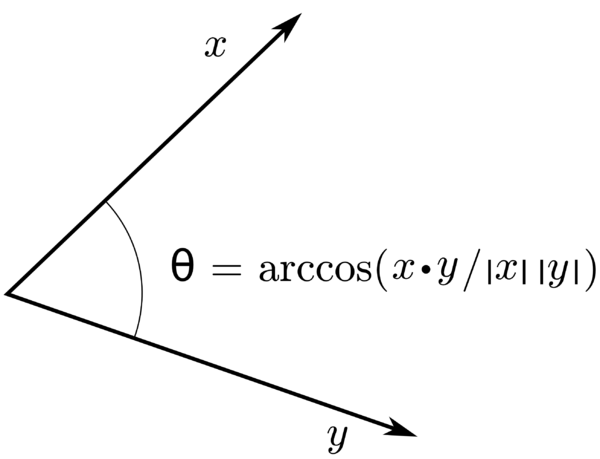
\includegraphics[scale=0.4]{figures/Inner_product_angle.png}
              
 \end{figure}


\end{frame}
%----------------------------------------------------------------------%
\begin{frame}
\frametitle{Word Embedding }
\begin{itemize}



\item Words with male connotations – e.g. male first names – are going to be positively correlated with \texttt{man - woman}.
\medskip
\item Female words, in turn, will be negatively correlated with the dimension.
\medskip
\item This framework provides an intuitive approach to measuring stereotypical associations in a given corpus. 
\medskip
\item Bolukbasi et al (2016) is a nice example
\end{itemize}

 \end{frame}
%----------------------------------------------------------------------%
\begin{frame}
\frametitle{Word Embedding: Example 1 }


  \begin{figure}[H] \centering
            \captionsetup{justification=centering}
              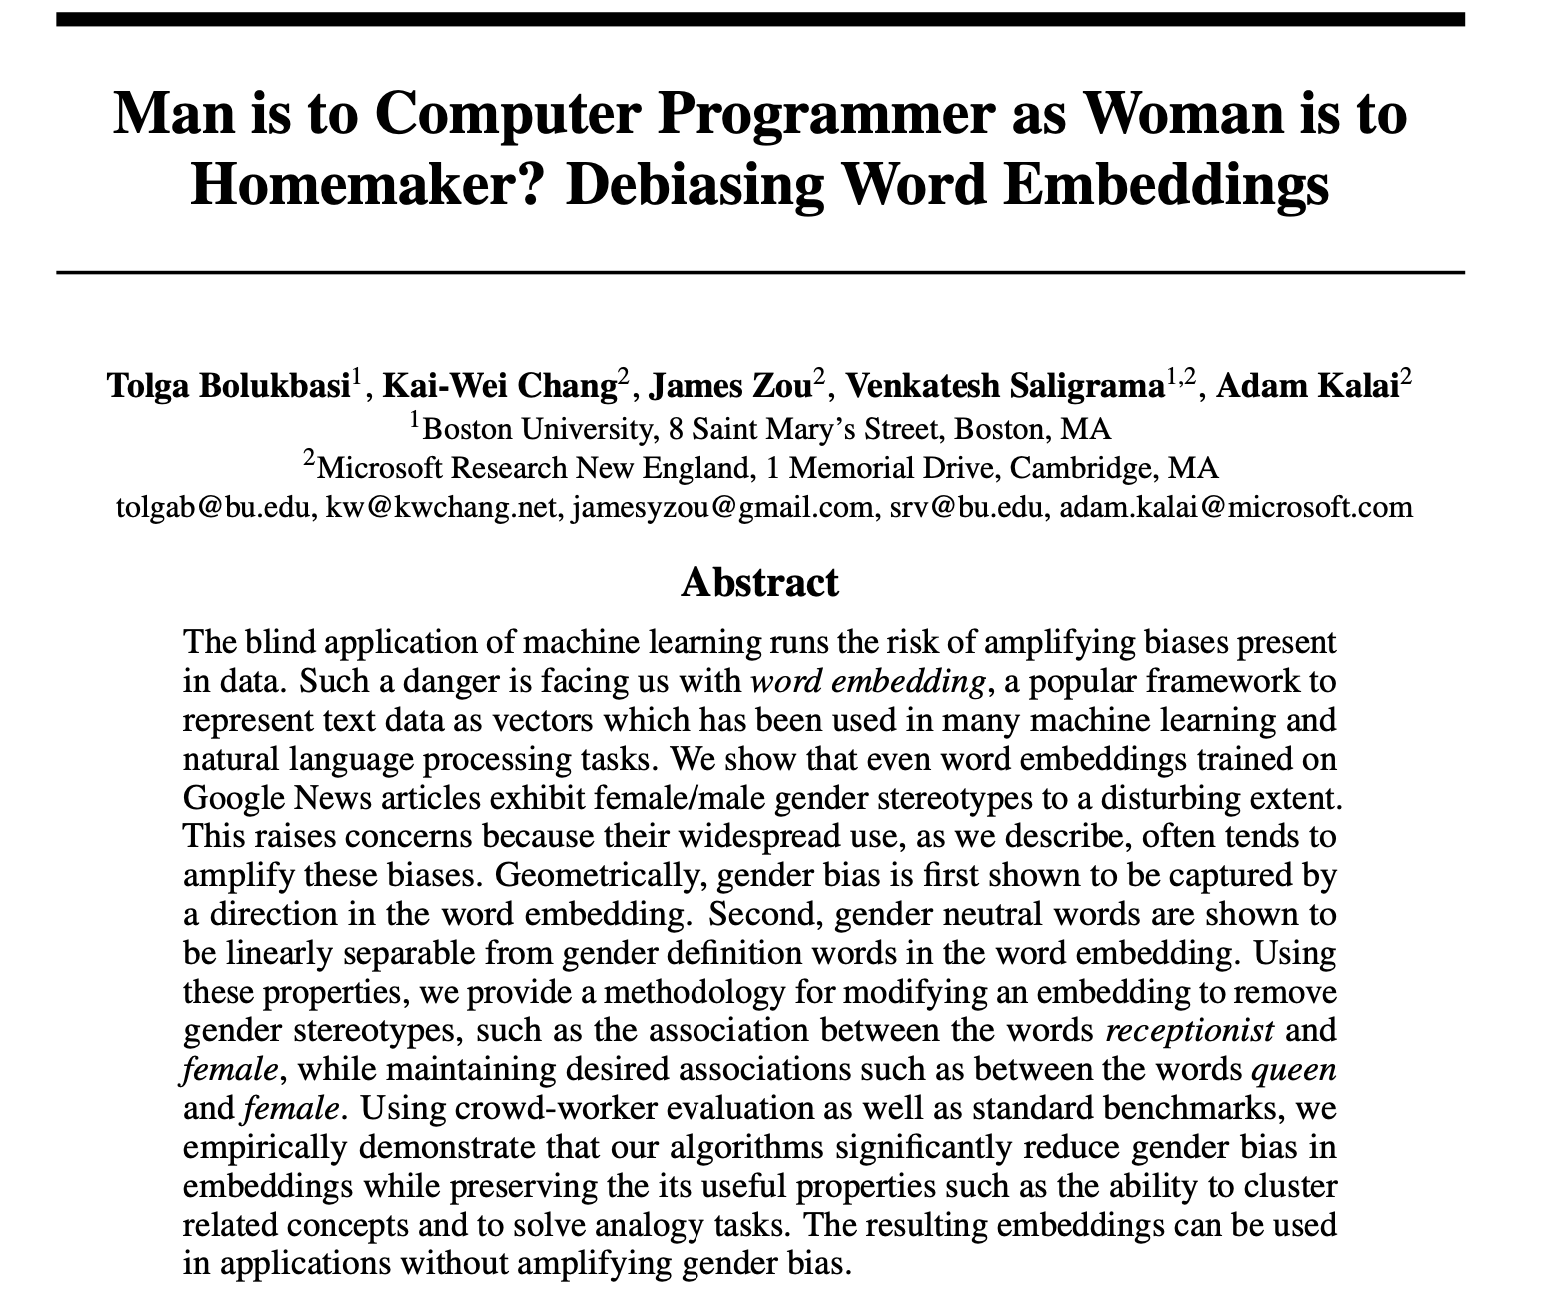
\includegraphics[scale=0.4]{figures/bolukbasi}
              
 \end{figure}

 \end{frame}
%----------------------------------------------------------------------%
\begin{frame}
\frametitle{Word Embedding: Example 1 }

\begin{itemize}


\item They trained a standard word2vec embedding algorithm on the Google News corpora of news articles. 
\item Then look at the differences between established gender words (for example, the vector for man minus the vector for woman, or father minus mother) to establish an axis in the embedding space that spans from masculinity to femininity. 
\item They then calculate the location along this axis for a large number of terms that should be gender-neutral. 
\item  The embedding space has learned—from how the words are used in news articles—that these professions are stereotypically viewed as female and male occupations.
\end{itemize}

\end{frame}
%----------------------------------------------------------------------%
\begin{frame}
\frametitle{Word Embedding: Example 1 }


  \begin{figure}[H] \centering
            \captionsetup{justification=centering}
              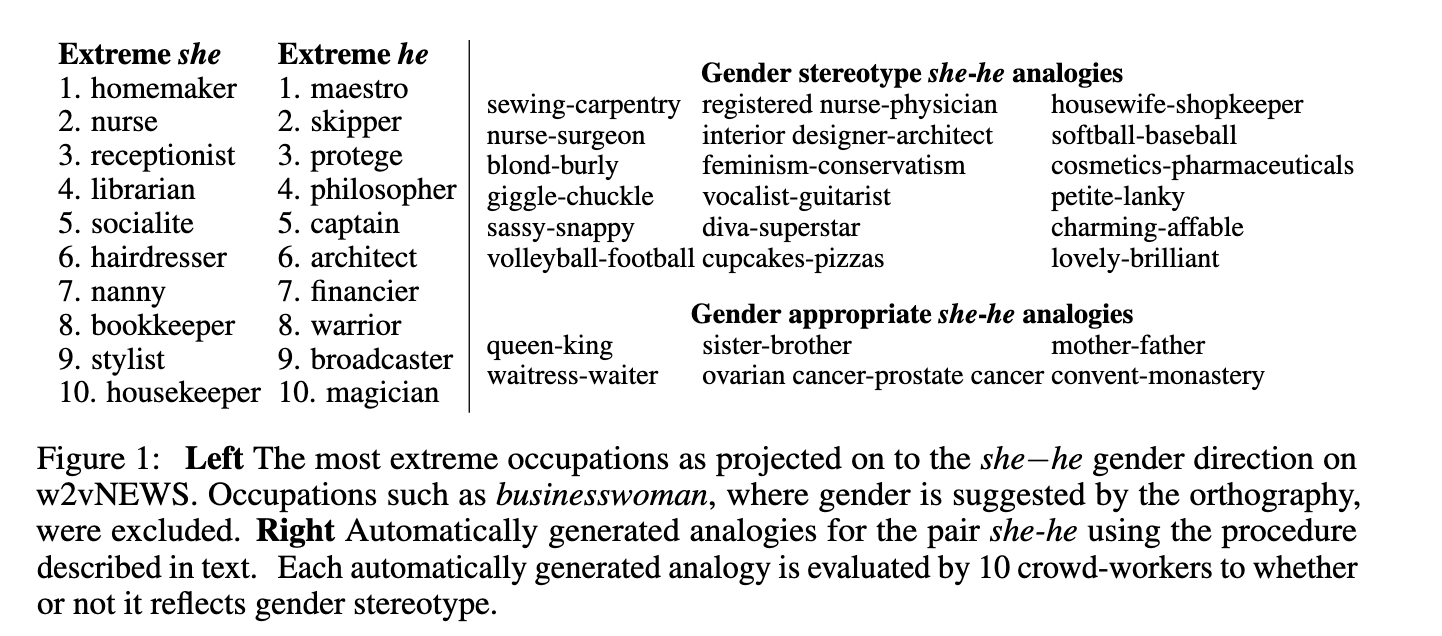
\includegraphics[scale=0.5]{figures/bolukbasi_2}
              
 \end{figure}

\end{frame}

%----------------------------------------------------------------------%
\begin{frame}
\frametitle{Word Embedding: Example 2 }


  \begin{figure}[H] \centering
            \captionsetup{justification=centering}
              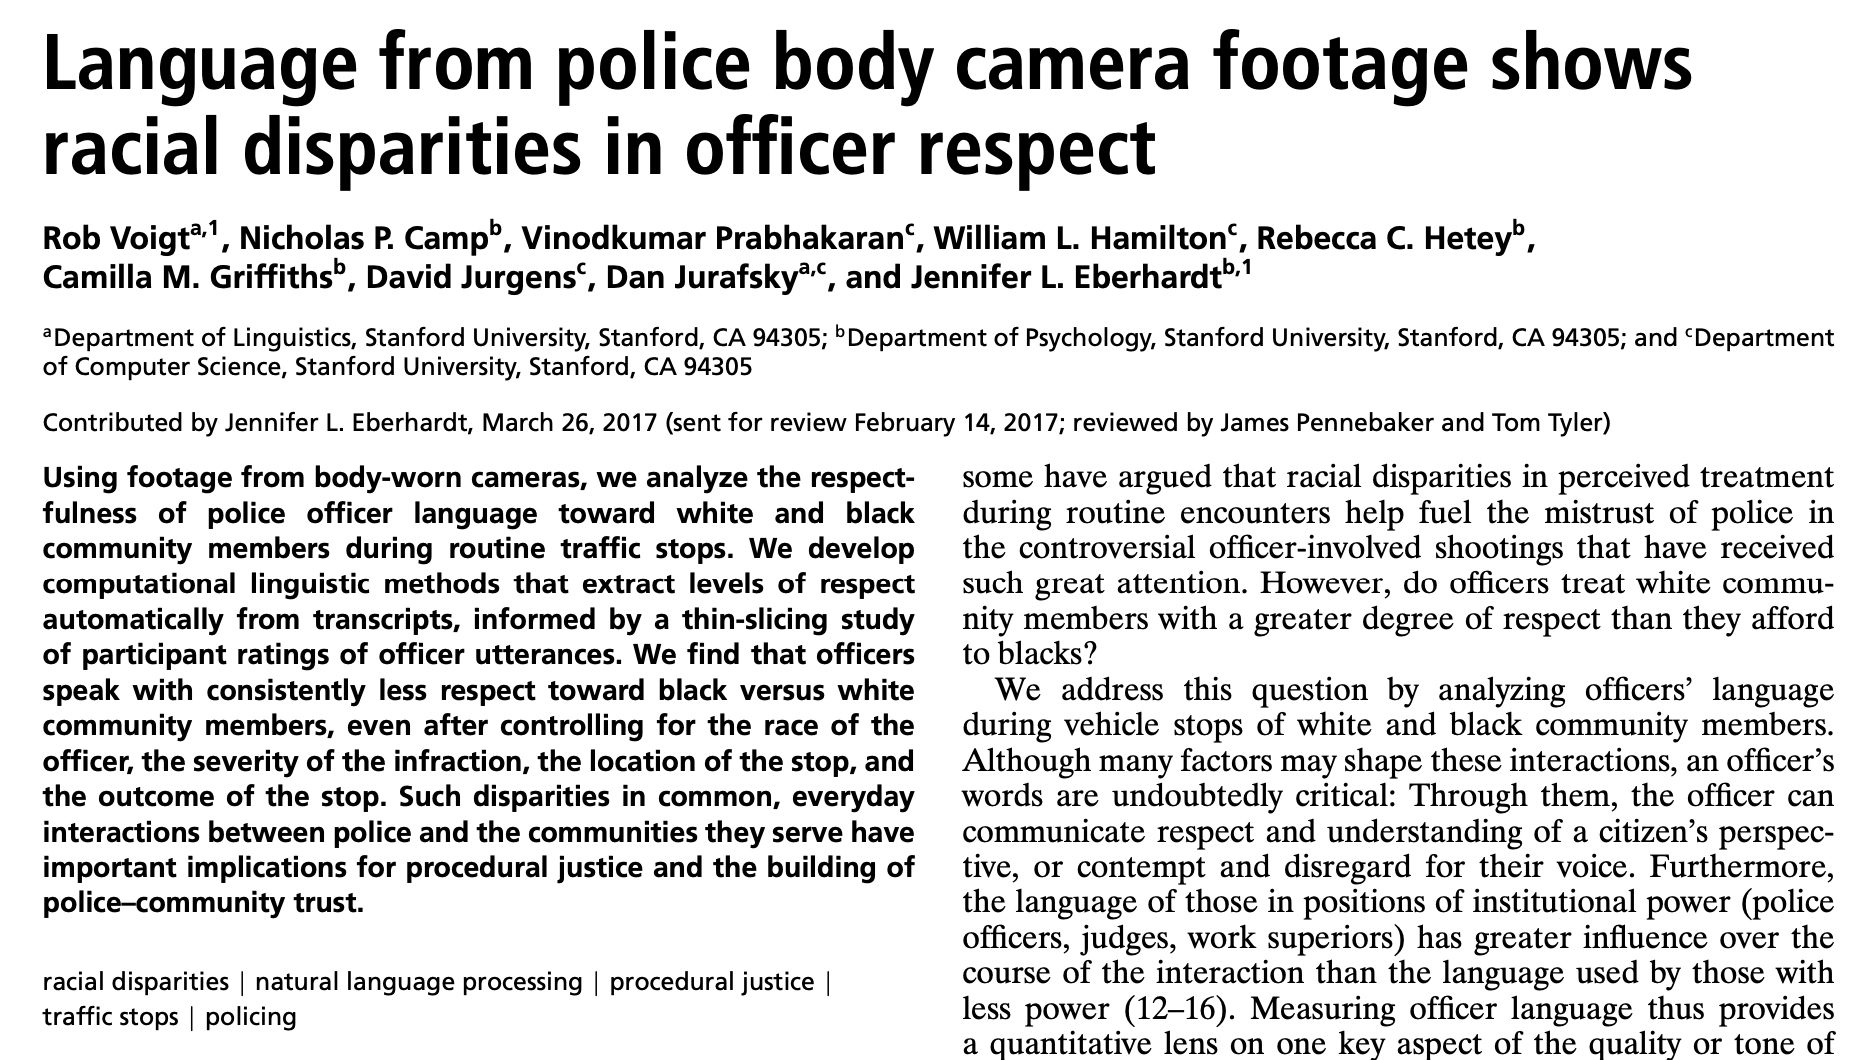
\includegraphics[scale=0.4]{figures/body_camera}
              
 \end{figure}

\end{frame}
%----------------------------------------------------------------------%
\begin{frame}
\frametitle{Word Embedding: Example 3 }


  \begin{figure}[H] \centering
            \captionsetup{justification=centering}
              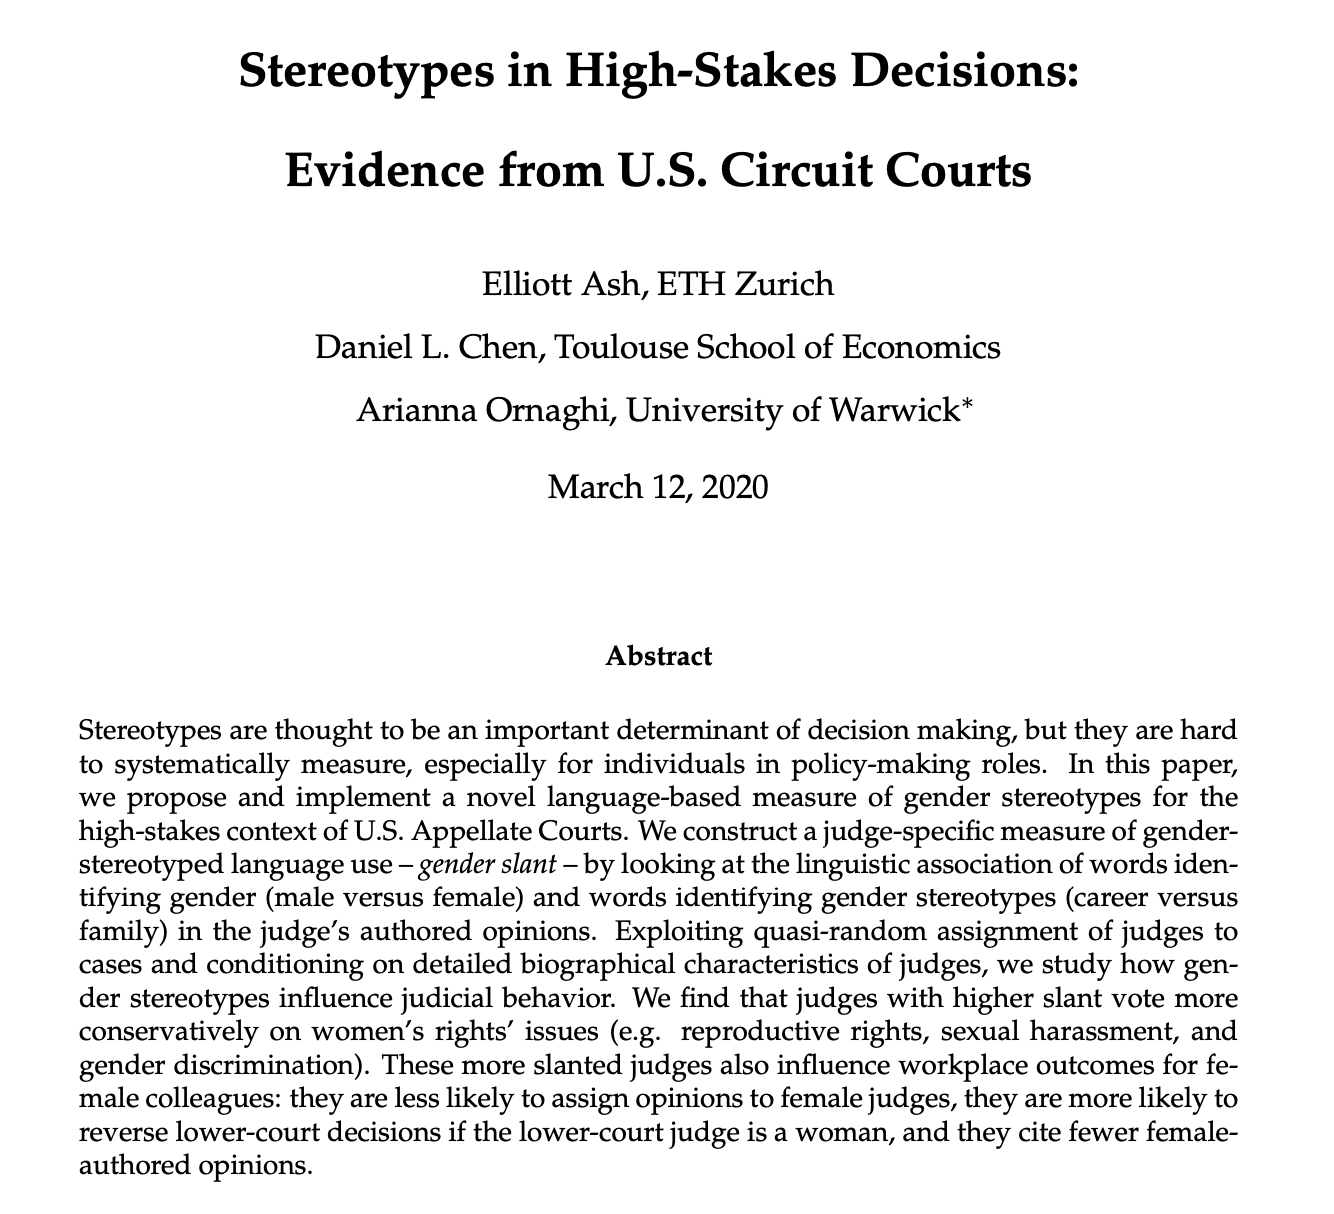
\includegraphics[scale=0.35]{figures/high_stakes_decisions}
              
 \end{figure}

\end{frame}
%----------------------------------------------------------------------%
\begin{frame}[fragile]
\frametitle{Word Embedding: Demo }


\begin{scriptsize}

\begin{Shaded}
\begin{Highlighting}[]
\KeywordTok{library}\NormalTok{(text2vec)}
\KeywordTok{load}\NormalTok{(}\StringTok{\textquotesingle{}shakes\_words\_df\_4text2vec.RData\textquotesingle{}}\NormalTok{)}
\KeywordTok{head}\NormalTok{(shakes\_words)}
\end{Highlighting}
\end{Shaded}

\end{scriptsize}
\begin{tiny}


\begin{verbatim}
##                    id         word
## 1 A_Lover_s_Complaint          nor
## 2 A_Lover_s_Complaint        gives
## 3 A_Lover_s_Complaint           it
## 4 A_Lover_s_Complaint satisfaction
## 5 A_Lover_s_Complaint           to
\end{verbatim}
\end{tiny}

\begin{scriptsize}

\begin{Shaded}
\begin{Highlighting}[]
\NormalTok{shakes\_words\_ls \textless{}{-}}\StringTok{ }\KeywordTok{list}\NormalTok{(shakes\_words}\OperatorTok{$}\NormalTok{word)}
\NormalTok{it \textless{}{-}}\StringTok{ }\KeywordTok{itoken}\NormalTok{(shakes\_words\_ls, }\DataTypeTok{progressbar =} \OtherTok{FALSE}\NormalTok{)}
\NormalTok{shakes\_vocab \textless{}{-}}\StringTok{ }\KeywordTok{create\_vocabulary}\NormalTok{(it)}
\NormalTok{shakes\_vocab \textless{}{-}}\StringTok{ }\KeywordTok{prune\_vocabulary}\NormalTok{(shakes\_vocab, }\DataTypeTok{term\_count\_min=} \DecValTok{5}\NormalTok{)}
\KeywordTok{head}\NormalTok{(shakes\_vocab)}
\end{Highlighting}
\end{Shaded}

\end{scriptsize}
\begin{tiny}


\begin{verbatim}
## Number of docs: 1 
## 0 stopwords:  ... 
## ngram_min = 1; ngram_max = 1 
## Vocabulary: 
##         term term_count doc_count
## 1:    abbess          5         1
## 2: abilities          5         1
## 3: accessary          5         1
## 4:       ace          5         1
## 5:    adders          5         1
\end{verbatim}
\end{tiny}

\end{frame}
%----------------------------------------------------------------------%
\begin{frame}[fragile]
\frametitle{Word Embedding: Demo }

\begin{itemize}
\item The next step is to create the token co-occurrence matrix (TCM). 
\item The definition of whether two words occur together is arbitrary. 
%\item Should we just look at previous and next word? Five behind and forward? This will definitely affect results so you will want to play around with it.
\end{itemize}

\begin{scriptsize}

\begin{Shaded}
\begin{Highlighting}[]
\CommentTok{\# maps words to indices}
\NormalTok{vectorizer \textless{}{-}}\StringTok{ }\KeywordTok{vocab\_vectorizer}\NormalTok{(shakes\_vocab)}

\CommentTok{\# use window of 10 for context words}
\NormalTok{shakes\_tcm \textless{}{-}}\StringTok{ }\KeywordTok{create\_tcm}\NormalTok{(it, vectorizer, }\DataTypeTok{skip\_grams\_window =} \DecValTok{10}\NormalTok{)}
\end{Highlighting}
\end{Shaded}
\end{scriptsize}



\begin{itemize}
\item Now we are ready to create the word vectors based on the GloVe model.
\end{itemize}


\begin{scriptsize}


\begin{Shaded}
\begin{Highlighting}[]
\NormalTok{glove \textless{}{-}}\StringTok{ }\NormalTok{GlobalVectors}\OperatorTok{$}\KeywordTok{new}\NormalTok{(}\DataTypeTok{rank =} \DecValTok{50}\NormalTok{, }\DataTypeTok{x\_max =} \DecValTok{10}\NormalTok{)}
\NormalTok{shakes\_wv\_main =}\StringTok{ }\NormalTok{glove}\OperatorTok{$}\KeywordTok{fit\_transform}\NormalTok{(shakes\_tcm, }\DataTypeTok{n\_iter =} \DecValTok{10}\NormalTok{, }\DataTypeTok{convergence\_tol =} \FloatTok{0.01}\NormalTok{, }\DataTypeTok{n\_threads =} \DecValTok{8}\NormalTok{)}
\end{Highlighting}
\end{Shaded}


\end{scriptsize}
\begin{tiny}


\begin{verbatim}
## INFO  [16:55:06.317] epoch 1, loss 0.1242 
## INFO  [16:55:08.764] epoch 2, loss 0.0844 
## INFO  [16:55:11.249] epoch 3, loss 0.0762 
## INFO  [16:55:13.680] epoch 4, loss 0.0707 
## INFO  [16:55:16.109] epoch 5, loss 0.0666 
## INFO  [16:55:18.540] epoch 6, loss 0.0634 
## INFO  [16:55:20.980] epoch 7, loss 0.0609 
## INFO  [16:55:23.419] epoch 8, loss 0.0589 
## INFO  [16:55:25.849] epoch 9, loss 0.0572 
## INFO  [16:55:28.288] epoch 10, loss 0.0558
\end{verbatim}
\end{tiny}
\end{frame}
%----------------------------------------------------------------------%
\begin{frame}[fragile]
\frametitle{Word Embedding: Demo }

\begin{scriptsize}

\begin{Shaded}
\begin{Highlighting}[]
\KeywordTok{dim}\NormalTok{(shakes\_wv\_main)}
\end{Highlighting}
\end{Shaded}
\end{scriptsize}
\begin{tiny}
\begin{verbatim}
## [1] 9094   50
\end{verbatim}
\end{tiny}

\begin{scriptsize}


\begin{Shaded}
\begin{Highlighting}[]
\NormalTok{shakes\_wv\_context \textless{}{-}}\StringTok{ }\NormalTok{glove}\OperatorTok{$}\NormalTok{components}

\KeywordTok{dim}\NormalTok{(shakes\_wv\_context)}
\end{Highlighting}
\end{Shaded}
\end{scriptsize}
\begin{tiny}

\begin{verbatim}
## [1]   50 9094
\end{verbatim}
\end{tiny}

\begin{scriptsize}


\begin{Shaded}
\begin{Highlighting}[]
\CommentTok{\# Either word{-}vectors matrices could work, but the developers of the technique}
\CommentTok{\# suggest the sum/mean may work better}
\NormalTok{shakes\_word\_vectors \textless{}{-}}\StringTok{ }\NormalTok{shakes\_wv\_main }\OperatorTok{+}\StringTok{ }\KeywordTok{t}\NormalTok{(shakes\_wv\_context)}

\NormalTok{rom \textless{}{-}}\StringTok{ }\NormalTok{shakes\_word\_vectors[}\StringTok{"romeo"}\NormalTok{, , drop =}\StringTok{ }\NormalTok{F]}

\NormalTok{cos\_sim\_rom \textless{}{-}}\StringTok{ }\KeywordTok{sim2}\NormalTok{(}\DataTypeTok{x =}\NormalTok{shakes\_word\_vectors, }\DataTypeTok{y =}\NormalTok{ rom, }\DataTypeTok{method =} \StringTok{"cosine"}\NormalTok{, }\DataTypeTok{norm =} \StringTok{"l2"}\NormalTok{)}
\CommentTok{\# head(sort(cos\_sim\_rom[,1], decreasing \textless{}{-} T), 10)}
\end{Highlighting}
\end{Shaded}

\end{scriptsize}
\begin{tiny}

\begin{verbatim}
##     romeo    juliet    tybalt     nurse  benvolio  banished  
## 1.0000000 0.7712391 0.7575977 0.6697068 0.6517349 0.6436404  
\end{verbatim}
\end{tiny}


\end{frame}

%----------------------------------------------------------------------%
\begin{frame}[fragile]
\frametitle{Word Embedding: Demo }

\begin{scriptsize}


\begin{Shaded}
\begin{Highlighting}[]
\NormalTok{test \textless{}{-}}\StringTok{ }\NormalTok{shakes\_word\_vectors[}\StringTok{"romeo"}\NormalTok{, , drop =}\StringTok{ }\NormalTok{F] }\OperatorTok{{-}}
\StringTok{  }\NormalTok{shakes\_word\_vectors[}\StringTok{"mercutio"}\NormalTok{, , drop =}\StringTok{ }\NormalTok{F] }\OperatorTok{+}
\StringTok{  }\NormalTok{shakes\_word\_vectors[}\StringTok{"nurse"}\NormalTok{, , drop =}\StringTok{ }\NormalTok{F]}

\NormalTok{cos\_sim\_test \textless{}{-}}\StringTok{ }\KeywordTok{sim2}\NormalTok{(}\DataTypeTok{x =}\NormalTok{ shakes\_word\_vectors, }\DataTypeTok{y =}\NormalTok{ test, }\DataTypeTok{method =} \StringTok{"cosine"}\NormalTok{, }\DataTypeTok{norm =} \StringTok{"l2"}\NormalTok{)}
\KeywordTok{head}\NormalTok{(}\KeywordTok{sort}\NormalTok{(cos\_sim\_test[,}\DecValTok{1}\NormalTok{], }\DataTypeTok{decreasing =}\NormalTok{ T), }\DecValTok{10}\NormalTok{)}
\end{Highlighting}
\end{Shaded}
\end{scriptsize}
\begin{tiny}


\begin{verbatim}
##     nurse    juliet     romeo      lady    mother       bed         o      wife 
## 0.8904362 0.7584004 0.7179267 0.6440354 0.6374490 0.5880860 0.5756074 0.5638571 
##   capulet    dromio 
## 0.5520459 0.5507196
\end{verbatim}
\end{tiny}



\end{frame}

%----------------------------------------------------------------------%
\section{Deep Learning: Intro}
%----------------------------------------------------------------------%
\begin{frame}
\frametitle{Deep Learning: Intro}

\begin{itemize}
    \item Word Embedding uses neural nets, so let's turn to them
    \medskip
  \item Neural networks are simple models.
  \medskip
  \item Their strength lays in their simplicity because basic patterns facilitate fast training and computation. 
  \medskip
  \item The model has linear combinations of inputs that are passed through nonlinear activation functions called nodes (or, in reference to the human brain, neurons). 
  \medskip
  \item A set of nodes taking different weighted sums of the same inputs is called a layer, and
  \medskip
  \item  The output of one layer's nodes becomes input to the next layer. 
\end{itemize}

\end{frame}
%----------------------------------------------------------------------%
\begin{frame}
\frametitle{Deep Learning: Intro}
  
  \begin{itemize}
    \item Let's start with a familiar and simple model, the linear model
  
  \end{itemize}

\def\layersep{2.5cm}

\begin{align}
y = \beta_1 x_1 + \beta_2 x_2 + \beta_3 x_3 +\beta_4 x_4 +\beta_5 x_5 + u
\end{align}


\begin{figure}[H]
\centering

\begin{tikzpicture}[shorten >=1pt,->,draw=black!50, node distance=\layersep]
    \tikzstyle{every pin edge}=[<-,shorten <=1pt]
    \tikzstyle{neuron}=[circle,fill=black!25,minimum size=17pt,inner sep=0pt]
    \tikzstyle{input neuron}=[neuron, fill=green!50];
    \tikzstyle{output neuron}=[neuron, fill=red!50];
    \tikzstyle{annot} = [text width=4em, text centered]

    % Draw the input layer nodes
    \foreach \name / \y in {1,...,5}
    % This is the same as writing \foreach \name / \y in {1/1,2/2,3/3,4/4}
        \node[input neuron, pin=left:$x_\y$] (I-\name) at (0,-\y) {};

    % Draw the output layer node
    \node[output neuron,pin={[pin edge={->}]right:Output}, right of=I-3] (O) {};

    % Connect every node in the input layer with every node in the
    % hidden layer.
    

    % Connect every node in the hidden layer with the output layer
    \foreach \source in {1,...,5}
        \path (I-\source) edge (O);

\end{tikzpicture}
\end{figure}



\end{frame}
%----------------------------------------------------------------------%
\begin{frame}
\frametitle{Deep Learning: Parallel to Biology?}


  \begin{figure}[H] \centering
            \captionsetup{justification=centering}
              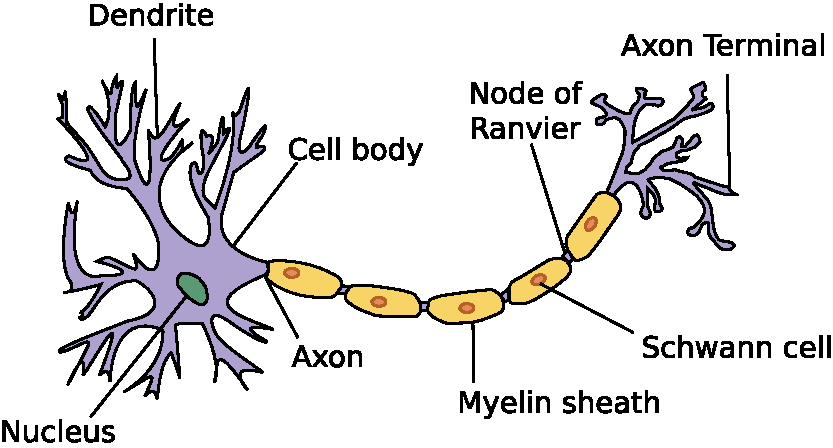
\includegraphics[scale=0.4]{figures/neuron.pdf}
              
 \end{figure}


\begin{itemize}
  \footnotesize
  \item Information $x_i$ arriving from other neurons (or environmental sensors such as the retina) is received in the dendrites. 
\item In particular, that information is weighted by synaptic weights $\beta_i$ determining the effect of the inputs (e.g., activation or inhibition via the product $x_i \beta_i$). 
\item The weighted inputs arriving from multiple sources are aggregated in the nucleus as a weighted sum $y=\sum_i x_i\beta_i$, and this information is then sent for further processing in the axon $y$

\item  From there it either reaches its destination (e.g., a muscle) or is fed into another neuron via its dendrites.


\end{itemize}


\end{frame}
%----------------------------------------------------------------------%
\begin{frame}
\frametitle{Deep Learning: Intro}

\begin{itemize} 
\item Linear Models May Go Wrong
\medskip
\begin{itemize}
\item For example, linearity implies the weaker assumption of monotonicity: that any increase in our feature must either always cause an increase in our model’s output (if the corresponding weight is positive), or always cause a decrease in our model’s output (if the corresponding weight is negative). 
\item But the world is highly non linear (trees work really well)
\end{itemize}
\medskip
\item We can incorporate hidden layers
\medskip
\item The simplest deep networks are called multilayer perceptrons, and they consist of multiple layers of neurons each fully connected to those in the layer below (from which they receive input) and those above (which they, in turn, influence). 

\end{itemize}
\end{frame}
%----------------------------------------------------------------------%
\begin{frame}
\frametitle{Deep Learning: Intro}



\def\layersep{2.5cm}

\begin{figure}[H]
\centering
\begin{tikzpicture}[shorten >=1pt,->,draw=black!50, node distance=\layersep]
    \tikzstyle{every pin edge}=[<-,shorten <=1pt]
    \tikzstyle{neuron}=[circle,fill=black!25,minimum size=17pt,inner sep=0pt]
    \tikzstyle{input neuron}=[neuron, fill=green!50];
    \tikzstyle{output neuron}=[neuron, fill=red!50];
    \tikzstyle{hidden neuron}=[neuron, fill=blue!50];
    \tikzstyle{annot} = [text width=4em, text centered]

    % Draw the input layer nodes
    \foreach \name / \y in {1,...,4}
    % This is the same as writing \foreach \name / \y in {1/1,2/2,3/3,4/4}
        \node[input neuron, pin=left:Input \#\y] (I-\name) at (0,-\y) {};

    % Draw the hidden layer nodes
    \foreach \name / \y in {1,...,5}
        \path[yshift=0.5cm]
            node[hidden neuron] (H-\name) at (\layersep,-\y cm) {};

    % Draw the output layer node
    \node[output neuron,pin={[pin edge={->}]right:Output}, right of=H-3] (O) {};

    % Connect every node in the input layer with every node in the
    % hidden layer.
    \foreach \source in {1,...,4}
        \foreach \dest in {1,...,5}
            \path (I-\source) edge (H-\dest);

    % Connect every node in the hidden layer with the output layer
    \foreach \source in {1,...,5}
        \path (H-\source) edge (O);

    % Annotate the layers
    \node[annot,above of=H-1, node distance=1cm] (hl) {Hidden layer};
    \node[annot,left of=hl] {Input layer};
    \node[annot,right of=hl] {Output layer};
\end{tikzpicture}
\end{figure}

\end{frame}
%----------------------------------------------------------------------%
\subsection{Demo}
%----------------------------------------------------------------------%
\begin{frame}[fragile]
\frametitle{Deep Learning: Demo}





\begin{Shaded}
\begin{Highlighting}[]
\KeywordTok{library}\NormalTok{(keras)}
\NormalTok{fashion\_mnist \textless{}{-}}\StringTok{ }\KeywordTok{dataset\_fashion\_mnist}\NormalTok{()}
\end{Highlighting}
\end{Shaded}

  \begin{figure}[H] \centering
            \captionsetup{justification=centering}
              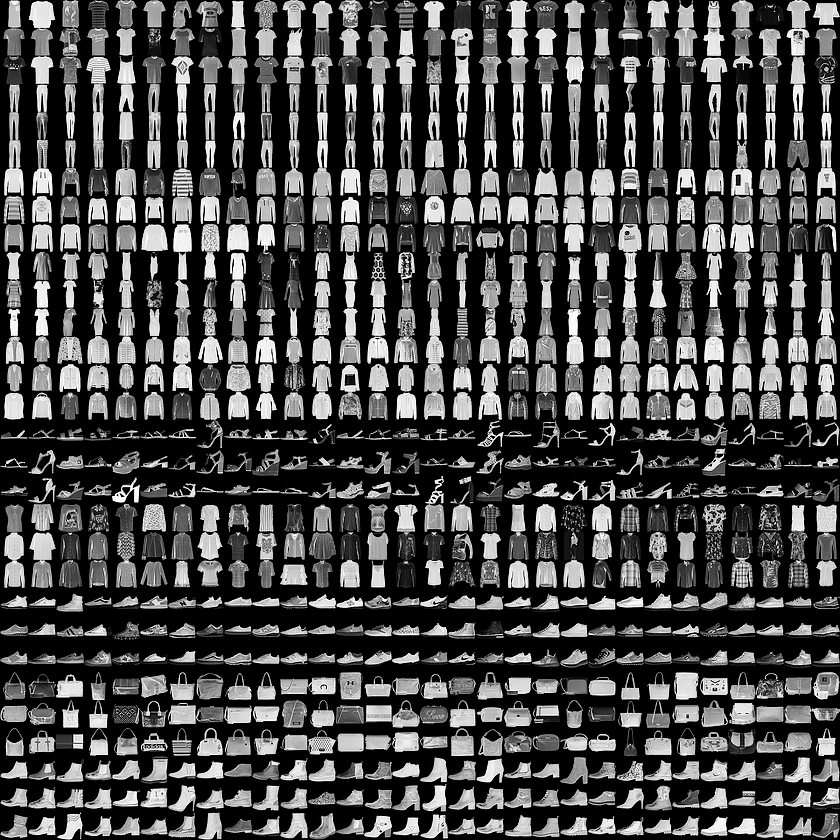
\includegraphics[scale=0.4]{figures/fashion-mnist-sprite}
              
 \end{figure}
\end{frame}
%----------------------------------------------------------------------%
\begin{frame}[fragile]
\frametitle{Deep Learning: Demo}

\begin{Shaded}
\begin{Highlighting}[]


\KeywordTok{c}\NormalTok{(train\_images, train\_labels) }\OperatorTok{\%\textless{}{-}\%}\StringTok{ }\NormalTok{fashion\_mnist}\OperatorTok{$}\NormalTok{train}
\KeywordTok{c}\NormalTok{(test\_images, test\_labels) }\OperatorTok{\%\textless{}{-}\%}\StringTok{ }\NormalTok{fashion\_mnist}\OperatorTok{$}\NormalTok{test}

\NormalTok{class\_names =}\StringTok{ }\KeywordTok{c}\NormalTok{(}\StringTok{\textquotesingle{}T{-}shirt/top\textquotesingle{}}\NormalTok{,}
                \StringTok{\textquotesingle{}Trouser\textquotesingle{}}\NormalTok{,}
                \StringTok{\textquotesingle{}Pullover\textquotesingle{}}\NormalTok{,}
                \StringTok{\textquotesingle{}Dress\textquotesingle{}}\NormalTok{,}
                \StringTok{\textquotesingle{}Coat\textquotesingle{}}\NormalTok{, }
                \StringTok{\textquotesingle{}Sandal\textquotesingle{}}\NormalTok{,}
                \StringTok{\textquotesingle{}Shirt\textquotesingle{}}\NormalTok{,}
                \StringTok{\textquotesingle{}Sneaker\textquotesingle{}}\NormalTok{,}
                \StringTok{\textquotesingle{}Bag\textquotesingle{}}\NormalTok{,}
                \StringTok{\textquotesingle{}Ankle boot\textquotesingle{}}\NormalTok{)}
\end{Highlighting}
\end{Shaded}

\end{frame}
%----------------------------------------------------------------------%
\begin{frame}[fragile]
\frametitle{Deep Learning: Demo}
\begin{scriptsize}

\begin{Shaded}
\begin{Highlighting}[]
\KeywordTok{library}\NormalTok{(tidyr)}
\KeywordTok{library}\NormalTok{(ggplot2)}

\NormalTok{image\_}\DecValTok{1}\NormalTok{ \textless{}{-}}\StringTok{ }\KeywordTok{as.data.frame}\NormalTok{(train\_images[}\DecValTok{1}\NormalTok{, , ])}
\KeywordTok{colnames}\NormalTok{(image\_}\DecValTok{1}\NormalTok{) \textless{}{-}}\StringTok{ }\KeywordTok{seq\_len}\NormalTok{(}\KeywordTok{ncol}\NormalTok{(image\_}\DecValTok{1}\NormalTok{))}
\NormalTok{image\_}\DecValTok{1}\OperatorTok{$}\NormalTok{y \textless{}{-}}\StringTok{ }\KeywordTok{seq\_len}\NormalTok{(}\KeywordTok{nrow}\NormalTok{(image\_}\DecValTok{1}\NormalTok{))}
\NormalTok{image\_}\DecValTok{1}\NormalTok{ \textless{}{-}}\StringTok{ }\KeywordTok{gather}\NormalTok{(image\_}\DecValTok{1}\NormalTok{, }\StringTok{"x"}\NormalTok{, }\StringTok{"value"}\NormalTok{, }\OperatorTok{{-}}\NormalTok{y)}
\NormalTok{image\_}\DecValTok{1}\OperatorTok{$}\NormalTok{x \textless{}{-}}\StringTok{ }\KeywordTok{as.integer}\NormalTok{(image\_}\DecValTok{1}\OperatorTok{$}\NormalTok{x)}

\KeywordTok{ggplot}\NormalTok{(image\_}\DecValTok{1}\NormalTok{, }\KeywordTok{aes}\NormalTok{(}\DataTypeTok{x =}\NormalTok{ x, }\DataTypeTok{y =}\NormalTok{ y, }\DataTypeTok{fill =}\NormalTok{ value)) }\OperatorTok{+}
\StringTok{  }\KeywordTok{geom\_tile}\NormalTok{() }\OperatorTok{+}
\StringTok{  }\KeywordTok{scale\_fill\_gradient}\NormalTok{(}\DataTypeTok{low =} \StringTok{"white"}\NormalTok{, }\DataTypeTok{high =} \StringTok{"black"}\NormalTok{, }\DataTypeTok{na.value =} \OtherTok{NA}\NormalTok{) }\OperatorTok{+}
\StringTok{  }\KeywordTok{scale\_y\_reverse}\NormalTok{() }\OperatorTok{+}
\StringTok{  }\KeywordTok{theme\_minimal}\NormalTok{() }\OperatorTok{+}
\StringTok{  }\KeywordTok{theme}\NormalTok{(}\DataTypeTok{panel.grid =} \KeywordTok{element\_blank}\NormalTok{())   }\OperatorTok{+}
\StringTok{  }\KeywordTok{theme}\NormalTok{(}\DataTypeTok{aspect.ratio =} \DecValTok{1}\NormalTok{) }\OperatorTok{+}
\StringTok{  }\KeywordTok{xlab}\NormalTok{(}\StringTok{""}\NormalTok{) }\OperatorTok{+}
\StringTok{  }\KeywordTok{ylab}\NormalTok{(}\StringTok{""}\NormalTok{)}
\end{Highlighting}
\end{Shaded}

\end{scriptsize}
\end{frame}
%----------------------------------------------------------------------%
\begin{frame}[fragile]
\frametitle{Deep Learning: Demo}
  \begin{figure}[H] \centering
            \captionsetup{justification=centering}
              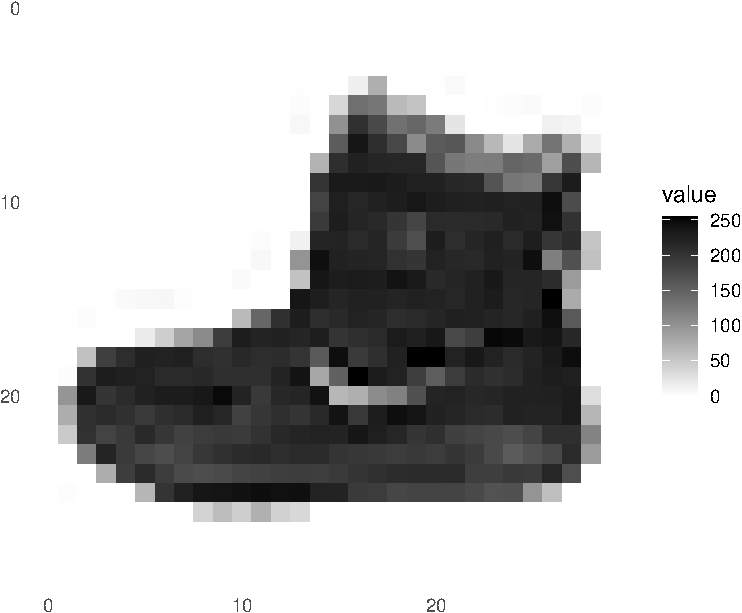
\includegraphics[scale=0.4]{figures/unnamed-chunk-3-1.pdf}
              
 \end{figure}


\end{frame}
%----------------------------------------------------------------------%
\begin{frame}[fragile]
\frametitle{Deep Learning: Demo}

\begin{Shaded}
\begin{Highlighting}[]
\NormalTok{train\_images \textless{}{-}}\StringTok{ }\NormalTok{train\_images }\OperatorTok{/}\StringTok{ }\DecValTok{255}
\NormalTok{test\_images \textless{}{-}}\StringTok{ }\NormalTok{test\_images }\OperatorTok{/}\StringTok{ }\DecValTok{255}
\end{Highlighting}
\end{Shaded}

\begin{Shaded}
\begin{Highlighting}[]
\KeywordTok{par}\NormalTok{(}\DataTypeTok{mfcol=}\KeywordTok{c}\NormalTok{(}\DecValTok{5}\NormalTok{,}\DecValTok{5}\NormalTok{))}
\KeywordTok{par}\NormalTok{(}\DataTypeTok{mar=}\KeywordTok{c}\NormalTok{(}\DecValTok{0}\NormalTok{, }\DecValTok{0}\NormalTok{, }\FloatTok{1.5}\NormalTok{, }\DecValTok{0}\NormalTok{), }\DataTypeTok{xaxs=}\StringTok{\textquotesingle{}i\textquotesingle{}}\NormalTok{, }\DataTypeTok{yaxs=}\StringTok{\textquotesingle{}i\textquotesingle{}}\NormalTok{)}
\ControlFlowTok{for}\NormalTok{ (i }\ControlFlowTok{in} \DecValTok{1}\OperatorTok{:}\DecValTok{25}\NormalTok{) \{ }
\NormalTok{  img \textless{}{-}}\StringTok{ }\NormalTok{train\_images[i, , ]}
\NormalTok{  img \textless{}{-}}\StringTok{ }\KeywordTok{t}\NormalTok{(}\KeywordTok{apply}\NormalTok{(img, }\DecValTok{2}\NormalTok{, rev)) }
  \KeywordTok{image}\NormalTok{(}\DecValTok{1}\OperatorTok{:}\DecValTok{28}\NormalTok{, }\DecValTok{1}\OperatorTok{:}\DecValTok{28}\NormalTok{, img, }\DataTypeTok{col =} \KeywordTok{gray}\NormalTok{((}\DecValTok{0}\OperatorTok{:}\DecValTok{255}\NormalTok{)}\OperatorTok{/}\DecValTok{255}\NormalTok{), }\DataTypeTok{xaxt =} \StringTok{\textquotesingle{}n\textquotesingle{}}\NormalTok{, }\DataTypeTok{yaxt =} \StringTok{\textquotesingle{}n\textquotesingle{}}\NormalTok{,}
        \DataTypeTok{main =} \KeywordTok{paste}\NormalTok{(class\_names[train\_labels[i] }\OperatorTok{+}\StringTok{ }\DecValTok{1}\NormalTok{]))}
\NormalTok{\}}
\end{Highlighting}
\end{Shaded}

\end{frame}
%----------------------------------------------------------------------%
\begin{frame}[fragile]
\frametitle{Deep Learning: Demo}

  \begin{figure}[H] \centering
            \captionsetup{justification=centering}
              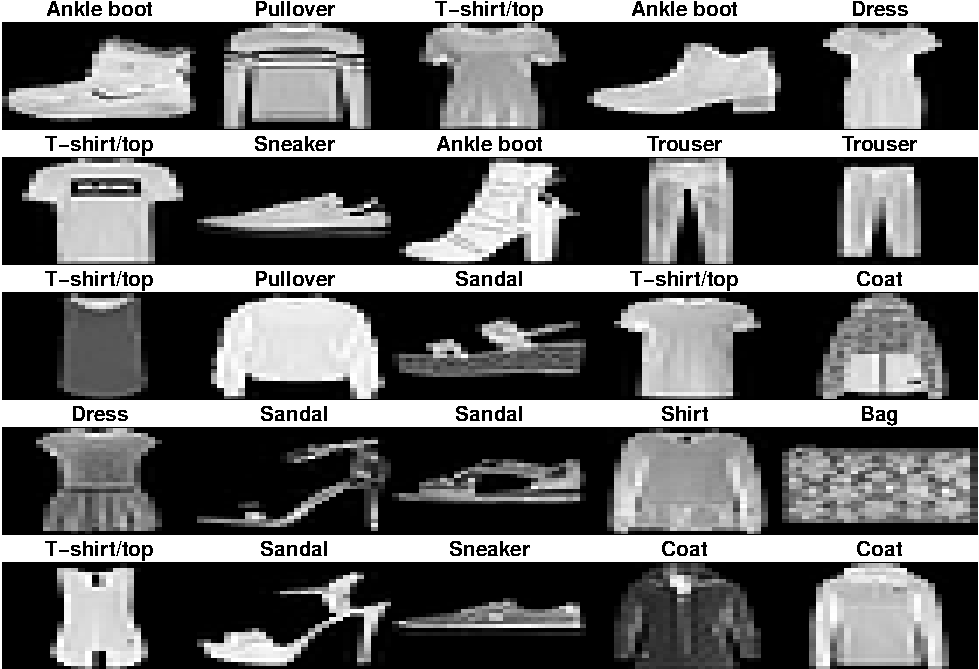
\includegraphics[scale=0.4]{figures/unnamed-chunk-5-1.pdf}
              
 \end{figure}

 \end{frame}
%----------------------------------------------------------------------%
\begin{frame}[fragile]
\frametitle{Deep Learning: Demo}


\begin{Shaded}
\begin{Highlighting}[]
\NormalTok{model \textless{}{-}}\StringTok{ }\KeywordTok{keras\_model\_sequential}\NormalTok{()}
\NormalTok{model }\OperatorTok{\%\textgreater{}\%}
\StringTok{  }\KeywordTok{layer\_flatten}\NormalTok{(}\DataTypeTok{input\_shape =} \KeywordTok{c}\NormalTok{(}\DecValTok{28}\NormalTok{, }\DecValTok{28}\NormalTok{)) }\OperatorTok{\%\textgreater{}\%}
\StringTok{  }\KeywordTok{layer\_dense}\NormalTok{(}\DataTypeTok{units =} \DecValTok{128}\NormalTok{, }\DataTypeTok{activation =} \StringTok{\textquotesingle{}relu\textquotesingle{}}\NormalTok{) }\OperatorTok{\%\textgreater{}\%}
\StringTok{  }\KeywordTok{layer\_dense}\NormalTok{(}\DataTypeTok{units =} \DecValTok{10}\NormalTok{, }\DataTypeTok{activation =} \StringTok{\textquotesingle{}softmax\textquotesingle{}}\NormalTok{)}
\end{Highlighting}
\end{Shaded}

\begin{Shaded}
\begin{Highlighting}[]
\NormalTok{model }\OperatorTok{\%\textgreater{}\%}\StringTok{ }\KeywordTok{compile}\NormalTok{(}
  \DataTypeTok{optimizer =} \StringTok{\textquotesingle{}adam\textquotesingle{}}\NormalTok{, }
  \DataTypeTok{loss =} \StringTok{\textquotesingle{}sparse\_categorical\_crossentropy\textquotesingle{}}\NormalTok{,}
  \DataTypeTok{metrics =} \KeywordTok{c}\NormalTok{(}\StringTok{\textquotesingle{}accuracy\textquotesingle{}}\NormalTok{)}
\NormalTok{)}
\NormalTok{model }\OperatorTok{\%\textgreater{}\%}\StringTok{ }\KeywordTok{fit}\NormalTok{(train\_images, train\_labels, }\DataTypeTok{epochs =} \DecValTok{5}\NormalTok{, }\DataTypeTok{verbose =} \DecValTok{2}\NormalTok{)}
\end{Highlighting}
\end{Shaded}

\end{frame}
%----------------------------------------------------------------------%
\begin{frame}[fragile]
\frametitle{Deep Learning: Demo}
\begin{scriptsize}
\begin{verbatim}
## Epoch 1/5
## 1875/1875 - 2s - loss: 0.5003 - accuracy: 0.8238
## Epoch 2/5
## 1875/1875 - 2s - loss: 0.3782 - accuracy: 0.8643
## Epoch 3/5
## 1875/1875 - 2s - loss: 0.3362 - accuracy: 0.8784
## Epoch 4/5
## 1875/1875 - 2s - loss: 0.3141 - accuracy: 0.8844
## Epoch 5/5
## 1875/1875 - 2s - loss: 0.2934 - accuracy: 0.8922
\end{verbatim}
\end{scriptsize}

\begin{Shaded}
\begin{Highlighting}[]
\NormalTok{score \textless{}{-}}\StringTok{ }\NormalTok{model }\OperatorTok{\%\textgreater{}\%}\StringTok{ }\KeywordTok{evaluate}\NormalTok{(test\_images, test\_labels, }\DataTypeTok{verbose =} \DecValTok{0}\NormalTok{)}

\KeywordTok{cat}\NormalTok{(}\StringTok{\textquotesingle{}Test loss:\textquotesingle{}}\NormalTok{, score[}\DecValTok{1}\NormalTok{], }\StringTok{"}\CharTok{\textbackslash{}n}\StringTok{"}\NormalTok{)}
\end{Highlighting}
\end{Shaded}
\begin{scriptsize}

\begin{verbatim}
## Test loss: 0.3377942

## Test accuracy: 0.8792
\end{verbatim}
\end{scriptsize}
\end{frame}
%----------------------------------------------------------------------%
\section{Review
 \& Next Steps}
%----------------------------------------------------------------------%
\begin{frame}
\frametitle{Review \& Next Steps}
  
\begin{itemize} 
  
\item  Word Embedding
\item  Word Embedding: Demo
\item  Deep Learning: Intro
\item  Deep Learning: Demo

    \bigskip  
  \item  Next class:  More on Neural Nets


\bigskip  
\item Questions? Questions about software? 

\end{itemize}
\end{frame}


%----------------------------------------------------------------------%
\section{Further Readings}
%----------------------------------------------------------------------%
\begin{frame}
\frametitle{Further Readings}

\begin{itemize}
\footnotesize

  \item Ash, E., Chen, D. L., \& Ornaghi, A. (2020). Stereotypes in High-Stakes Decisions: Evidence from US Circuit Courts (No. 1256). University of Warwick, Department of Economics.
  \medskip
  \item Aston Zhang, Zachary C. Lipton, Mu Li, and Alexander J. Smola (2020) Dive into Deep Learning. Release 0.15.1. \url{http://d2l.ai/index.html}
  \medskip
  \item Bolukbasi, T., Chang, K. W., Zou, J. Y., Saligrama, V., \& Kalai, A. T. (2016). Man is to computer programmer as woman is to homemaker? debiasing word embeddings. In Advances in neural information processing systems (pp. 4349-4357).
  \medskip
  \item Clark, M (2018). An Introduction to Text Processing and Analysis with R. \url{https://m-clark.github.io/text-analysis-with-R/}
  \medskip
  Rstudio (2020). Tutorial TensorFlow \url{https://tensorflow.rstudio.com/tutorials/beginners/basic-ml/tutorial_basic_classification/}
  \medskip
  \item Taddy, M. (2019). Business data science: Combining machine learning and economics to optimize, automate, and accelerate business decisions. McGraw Hill Professional.
  \medskip
  \item Voigt, R., Camp, N. P., Prabhakaran, V., Hamilton, W. L., Hetey, R. C., Griffiths, C. M., ... \& Eberhardt, J. L. (2017). Language from police body camera footage shows racial disparities in officer respect. Proceedings of the National Academy of Sciences, 114(25), 6521-6526.

  
\end{itemize}

\end{frame}
%----------------------------------------------------------------------%
%----------------------------------------------------------------------%
\end{document}
%----------------------------------------------------------------------%
%----------------------------------------------------------------------%
